\section{Algoritmi di guida}

%\begin{idee}
%	\cite{ElikerKaram2018AOPf}
%	\cite{baseTesi}
%	\cite{Mendoza-SotoJoséLuis2018Cgpc}
%	\cite{PathPlannigOverview}
%	
%	
%	\cite{YangLiang2016SoR3} : 
%	
%	La necessità è quella di avere autonomia nello spostamento senza l'intervento dell'uomo, determinando autonomamente il percorso da seguire.
%	Tra gli obbiettivi di pianificazione del percorso c'è anche quello di evitare gli ostacoli possibili per questioni di sicurezza.
%	Nel contesto degli UAV il problema è un problema tridimensionale.
%	
%	La soluzione a questo tipo di problema è estremamente complessa.
%	
%	Si può suddividere il problema in 2 parti fondamentali:
%	
%	1. Percezione e modellazione dell'ambiente
%	2. Applicazione dell'algoritmo di pianificazione
%	
%	Non è necessario però che la pianificazione si sempre accompagnata da una ottimizazione, alcune volte basta che questa colleghi i due punti nello spazio.
%	Si distingue in pianificazione del persorso e pianificazione del percorso ottimo se si vuole ottimizzare una certa funzione di costo oppure no.
%	
%	Sussiste una differenza tra pianificazione del percorso e della traiettoria. La pianificazione del percorso cerca solo un a curva o una sequenza di curve che colleghino due punti nello spazio, mentre la pianificazione della traiettoria prevede di determinare anche come questa debba essere percorsa, descrivendo in modo cinematico e dinamico, attraverso la valutazione di questi nella ricerca della soluzione.
%	
%	Si possono classificare gli algoritmi di pianificazione dei percorsi in 5 categorie.
%	
%	1. Algoritmi basati sul campionamento:
%		Questi algoritmi richiedono la conoscenza a priori di informazioni sull'ambiente e una rappresentazione matematica di questo. Si prevede di dividere l'ambiente in nodi o celle o altre forme. Avviene poi una ricerca attraverso una ricerca casuale. Questa categoria si può suddividere a sua volta in altre 2 categorie : attive e passive. Attive  si intende algoritmi che esploraro rapidamente in modo casuale per trovare il percorso migliore. Passivi algoritmi che si occupano di cercare la soluzione da percorsi già presenti come su di una mappa.
%		Tra gli attivi si parla di Rapidly Exploring Random Tree (RRT). Si generano nodi casualmente nello spazio cercando di raggiungere il punto obbiettivo. L'algoritmo ha il problema però di essere molto lento se l'ambiente è disordinato per trovare la soluzione.
%		Dinamic Domain RRT (DDRRT) : questa evoluzione attraverso l'introduzione di sfere permette di velocizzare l'esplorazione dell'ambiente superando in parte la limitazione della versione RRT.
%		Rapidly Exploring Random Graph (RRG) : Per migliorare la soluzione ottenuta attraverso RRT e DDRRT viene introdotta una struttura dati che assiste l'esplorazione. Attraverso questo approccio nuovi collegamenti vengono fatti durante l'esplorazione per avere una soluzione migliorata. Ulteriore miglioramento può essere fatto utilizzando RRT-Star (RRT*) una versione in cui vengono eliminati i percorsi che si sono ottenuti e che probabilmente non sono ottimali , raffinando invece le connessioni che lo sono. In questo modo si ottiene una soluzione ottimizzata al prezzo però di non poter generare più percorsi contemporaneamente e un costo computazionale maggiore.
%		Probabilistic Road Map (PRM) genera i nodi in modo da avere un collegamento tra i due punti. Considera differenti scelte dal set di soluzioni che si possono trovare e attraverso un algoritmo di ricerca testa la soluzione per discriminare la migliore.
%		Vornoi: Attraverso l'uso dei digrammi di Voronoi si determinano i nodi e le connessioni per generare il percorso. Il vantaggio è che in questo approccio la minima distanza con gli ostacoli è sempre la stessa. Si continua a suddividere l'ambiente fino a quando si ottiene collegamento tra tutti i canali. Non è in grado di generare contemporaneamente il migliore percorso , per sopperire a questa limitazione è necessario utilizzare un algoritmo di ricerca per trovare la soluzione migliore.
%		Algoritmo basato su energia potenziale. Viene considerata una funzione potenziale attraverso interazione tra spazio percorribile e non, da questo si determina il percorso, è molto facile da implementare e ha un costo computazionale basso, ha però il problema di presentare minimi locali e punti di ristagno , limitazione però facilmente superabile in diversi modi.
%		Riassumendo questi approcci si basano sull'esplorazione delle possibili soluzioni e la successiva valutazione per migliorare la forma ottenuta. L'algoritmo si applica in modo indipendente all'ambiente specifico perché concettualmente separato avendo la capacità di determinare le collisioni in modo autonomo se nella ricerca avviene.
%	
%		
%	2. Algoritmi basati sui nodi
%		Questi algoritmi sono basati sull'utilizzo di nodi appartenenti ad un grafo scomposto, ricercando in mappe già pronte.
%		Algoritmo di Dijkstra.l Conoscendo già un grafo in cui gli archi e i nodi sono stati pesati , si attua una ricerca per ridurre la funzione di costo. Partendo quindi dai nodi si genera il grafo con i pesi e poi si applica l'algoritmo. Un evoluzione di questo algoritmo è A-Star (A*). Indroducendo una stima euristica del costo durante il processo di ricerca permetta una più veloce velocità di convergenza. Per applicazioni con ostacoli dinamici dsi utilizza una versione modificata denominata D-Star (D*) che prevede di modificare i pesi nel grafo in funzione della configurazione degli ostacoli. Questo tipo di approccio però è limitativo in termini di soluzioni a causa della chiara incompletezza della struttura di configurazioni nell'ambiente. Di fatto si parla solamente di un algoritmo di ricerca no è in grado di generare un percorso ma solo una configurazione di sotto-percorsi già precostituiti.
%		
%	3. Algoritmi basati su modelli matematici
%		Questi metodi modellano l'ambiente  e il sistema e il sistema e modellano la funzione di costo con i limiti e vincoli per ottenere la soluzione ottimale. Equazioni e disequazioni vengono utilizzate per ottenere la soluzione migliore.
%		Vengono descritte matematicamente i vincoli cinematici e dinamici attraverso combinazioni di forme polinomiali. Si può modelare sistemai tempovarianti. 
%		Algoritmi lineari. Si definisce una funzione di costo che contiene all'interno tutti i vincoli in termini di ottimizzazione della soluzione e sul e limitazioni del controllo che penalizza il costo. all'interno è presente anche l'espressione che descrive lo spazio effettivamente raggiungibile. Attraverso questa formulazione si descrive completamente l'ambiente. \'E possibile anche tenere conto delle incertezze e fattori di disturbo.
%		Controllo ottimo. Si imposta il problema da un pusto di vista ottimo per il controllollo utilizzando equazioni differenziali. Si utilizza una formulazione Hamiltoniana per risolvere il problema. 
%		Questi approcci descrivono completamente il lo stato e le variabili in gioco . Risultano però essere complessi e molto pesanti da risolvere.
%	
%	4. Algoritmi bio-ispirati
%		Questi algoritmi mimano la natura per trovare una soluzione al problema. L'approccio alla soluzione è stocastico superando la soluzione basata su modelli matematici per problemi molto complessi.
%		Si può fare una suddivisione in due sottocategorie: Algoritmi evoluzionistici e reti neurali.
%		Gli algortmi evoluzionistici cercano di imitare comportamenti e approcci presenti in naura ed osservati. Tra questi è famoso l'algoritmo genetico che attraverso una approccio simile alla selezione naturale determina attraverso simulazioni il migliore approccio da una famiglia.
%		Le reti neurali esattamente come descritto precedentemente sono formati da modelli matematici che imitano il funzionamento dei neuroni in layer. In questa applicazione specifica si fa riferimento ad una formulazione dinamica che tiene conto dell'attività del neurone.
%		
%	5. Algoritmi misti
%		Normalmente gli alg
%		oritmi presentati tendono a fondersi assieme per sopperire alle proprie limitazioni e trovare assieme una soluzione ottimale. Migliori soluzioni miste. Dove sono presenti delle limitazioni si interviene un altro algoritmo che supporta il primo a trovare una soluzione ottimale.	Si possono suddividere in due categorie: Embedded Multifusional Algorithms (EMA) e Ranked Multifusion. Algorithm (RMA).
%		EMA lavorano assieme sullo stesso modello.
%		RMA lavorano su livelli separati e in modo ordinato.	
%	
%\end{idee}

Per poter muovere correttamente il velivolo nello spazio senza l'ausilio del controllo da parte di un operatore umano, mantenendo le distanze di sicurezza e in modo compatibile alla sua dinamica e alle leggi di controllo implementate, occorre generare correttamente i segnali necessari. A questo scopo vengono sviluppate due funzionalità: trovare il percorso nello spazio evitando eventuali ostacoli presenti, creare i segnali necessari a seguire il percorso trovato seguendo vincoli di velocità e accelerazioni compatibili con le leggi di controllo e il velivolo stesso. Vengono quindi descritti gli algoritmi di pianificazione del percorso e della traiettoria in applicazioni tridimensionali presenti in letteratura \cite{YangLiang2016SoR3}, \cite{PathPlannigOverview}.

\subsection{Pianificazione del percorso}

La ricerca di un percorso evitando gli ostacoli in ambiente tridimensionale è un problema molto complesso. Per semplificare la trattazione si può suddividere il problema in 2 parti fondamentali:
\begin{itemize}
	\item Percezione e modellazione dell'ambiente
	\item Applicazione dell'algoritmo di pianificazione
\end{itemize}

Per descrivere correttamente le fasi necessarie alla guida del mezzo bisogna fare una distinzione concettuale tra pianificazione del percorso e pianificazione della traiettoria. La pianificazione del percorso ha come obbiettivo la sola ricerca di un collegamento geometrico nello spazio continuo o sequenziale, in modo da collegare il punto di partenza e di arrivo della pianificazione della missione. La pianificazione della traiettoria invece prevede di determinare come la precedente soluzione in termini geometrici debba essere percorsa, studiando attraverso la descrizione della cinematica e della dinamica del corpo. L'obbiettivo finale di quest'ultimo studio, rispettando i vincoli imposti determina in uscita la descrizione dei segnali di riferimento per la parte di comando vero e proprio, \cite{YangLiang2016SoR3}, \cite{PathPlannigOverview}.

Si possono classificare gli algoritmi di pianificazione dei percorsi in 5 categorie che vengono qui descritti brevemente.

\begin{figure}
	\centering
	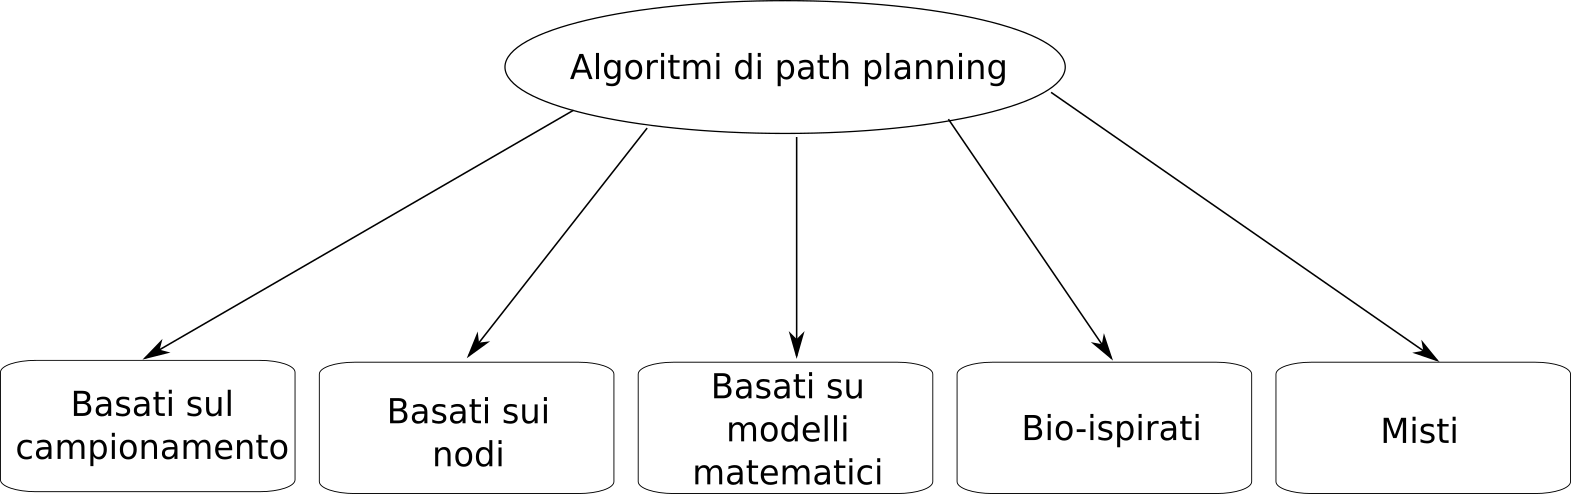
\includegraphics[width=0.7\textwidth]{SistemaQuadrirotore/Figure/Path}
	\caption{Classificazione dei tipi di algoritmi di Path Planning \cite{YangLiang2016SoR3}}
\end{figure}


\subsubsection{Algoritmi basati sul campionamento}

Gli algoritmi basati sul campionamento sono in grado di generare un percorso utile attraverso l'esplorazione casuale dell'ambiente. Fanno uso di concetti come nodi, celle o altre forme per determinare se il punto esplorato è compatibile con la soluzione da ricercare. Per effettuare la ricerca questo tipo di algoritmo necessitano di avere una conoscenza a priori dell'ambiente nella quale viene effettuata la ricerca.
Si possono suddividere le possibili implementazioni in due categorie:
\begin{itemize}
	\item \textbf{Attivi : } La soluzione avviene attraverso un esplorazione totalmente casuale di nuovi punti nella mappa in un solo passaggio si cerca di ottimizzarla
	\item \textbf{Passivi : }  La soluzione avviene attraverso la ricerca da un set di possibili soluzioni già determinate in un passaggio preliminare e attraverso un algoritmo di ricerca la migliore viene selezionata
\end{itemize}

%Questi algoritmi richiedono la conoscenza a priori di informazioni sull'ambiente e una rappresentazione matematica di questo. Si prevede di dividere l'ambiente in nodi o celle o altre forme. Avviene poi una ricerca attraverso una ricerca casuale. Questa categoria si può suddividere a sua volta in altre 2 categorie : attive e passive. Attive  si intende algoritmi che esploraro rapidamente in modo casuale per trovare il percorso migliore. Passivi algoritmi che si occupano di cercare la soluzione da percorsi già presenti come su di una mappa.



Nella categoria di algoritmi attivi ricade la Rapidly Exploring Random Tree (RRT). In questo algoritmo vengono generati nodi casualmente nello spazio con l'obbiettivo di raggiungere il punto obbiettivo dopo un numero non definito a priori di interazioni, \cite{Lavalle98rapidly-exploringrandom}. L'algoritmo ha il problema quindi di essere molto lento se l'ambiente è disordinato.

Per migliorare la velocità di convergenza ad una soluzione il precedente approccio viene arricchito nell'implementazione del Dinamic Domain RRT (DDRRT). In questo algoritmo attraverso l'introduzione di sfere attorno al nodo generato in ogni passaggio, si permette di determinare lo stato di esplorazione evitando di generare nodi in luoghi già esplorati, velocizzando il processo e superando in parte la limitazione della versione RRT, \cite{YangLiang2016SoR3}.

Generando una struttura dati ottimizzata per la ricerca utilizzando la Rapidly Exploring Random Graph (RRG), si può migliorare ulteriormente la l'approccio ottenuto attraverso RRT e DDRRT, velocizzando l'esplorazione. Il metodo prevede di generare ulteriori nodi intermedi, parallelizzando la generazione di percorsi alternativi attraverso il riempimento di un grafo di supporto, \cite{doi:10.1080/01691864.2013.805472}.

Esiste in bibliografia anche una versione ottimizzata della RRT, denominata RRT-Star (RRT*), \cite{ChoudhurySanjiban2013RSar}. Una versione in cui vengono eliminati i percorsi che si sono ottenuti e che probabilmente non sono ottimali, raffinando invece le connessioni, che vengono valutati dall'algoritmo  come migliori, di fatto una versione ad albero della RRG, \cite{YangLiang2016SoR3}. In questo modo si ottiene una soluzione ottimizzata rispetto agli altri algoritmi precedenti al prezzo però di non poter generare più percorsi contemporaneamente, utili per applicazioni con più robot, come mostrato nel lavoro \cite{doi:10.1080/01691864.2013.805472}. Questo approccio ha inoltre lo svantaggio di avere un costo computazione maggiore.

L'algoritmo Probabilistic Road Map (PRM) a differenza del RRT, prevede di generare più percorsi tra i vari nodi generati e valutarne successivamente la probabilità dell'efficacia di un percorso rispetto ad un altro. Attraverso un algoritmo di ricerca si testa la soluzione per discriminare la migliore, \cite{KavrakiL1994Prfp}.

Un approccio passivo è quello che viene definito Voronoi. Attraverso l'uso dei digrammi di Voronoi si determinano i nodi e le connessioni per generare il percorso. Il vantaggio è che in questo approccio si basa sulla minima distanza tra i nodi e con gli ostacoli. Si continua a suddividere l'ambiente fino a quando si ottiene collegamento tra tutti i segmenti che vengono man mano a formarsi, \cite{LuchnikovVA1999Vaov}. In questo approccio non è generare contemporaneamente il migliore percorso. Per sopperire a questa limitazione è necessario utilizzare in supporto un algoritmo di ricerca per discriminare il percorso migliore.

Tra i metodi attivi è presente anche l'algoritmo basato su energia potenziale. In questo algoritmo viene considerata una funzione potenziale attraverso interazione tra spazio percorribile e spazio occupato. Attraverso la generazione di una funzione potenziale funzione dell'ambiente e di pseudo forze si definisce il percorso da seguire. \'E molto facile da implementare e ha un costo computazionale basso, ha però il problema di presentare minimi locali e punti di ristagno , limitazione però facilmente superabile, \cite{RimonE1992Ernu}.

Riassumendo questi approcci si basano sull'esplorazione delle possibili soluzioni e la successiva valutazione per migliorare la forma ottenuta, sia in un solo passaggio che in più passaggi. L'algoritmo si applica in modo indipendente all'ambiente specifico, se non per la descrizione degli ostacoli e vincoli, aspetto concettualmente separato avendo la capacità di determinare le collisioni in modo autonomo, 
\cite{YangLiang2016SoR3}.


\subsubsection{Algoritmi basati sui nodi}
Questi algoritmi sono basati sull'utilizzo di nodi appartenenti ad un grafo scomposto, ricercando in mappe già pronte.

Tra questi algoritmi si trova l'algoritmo di Dijkstra, \cite{DIJKSTRA1959}. Conoscendo già un grafo in cui gli archi e i nodi sono stati pesati, si attua una ricerca per ridurre la funzione di costo. Partendo quindi dai nodi si genera il grafo con i pesi e poi si applica l'algoritmo. 

Un evoluzione di questo algoritmo è A-Star (A*), \cite{HartPeter1968AFBf}. Introducendo una stima euristica del costo durante il processo di ricerca si ottiene una più veloce velocità di convergenza. Per applicazioni con ostacoli dinamici si utilizza una versione modificata denominata D-Star (D*) che prevede di modificare i pesi nel grafo in funzione della configurazione degli ostacoli. 

Questo tipo di approccio però è limitativo in termini di soluzioni a causa della chiara incompletezza della struttura di configurazioni nell'ambiente. Di fatto si parla solamente di un algoritmo di ricerca non è in grado di generare un percorso ma solo una configurazione di sotto-percorsi già precostituiti, \cite{StentzA1994Oaep}, \cite{YangLiang2016SoR3}.

\subsubsection{Algoritmi basati su modelli matematici}
Questi metodi modellano l'ambiente  e il sistema modellando la funzione di costo con i limiti e vincoli per ottenere la soluzione ottimale. Equazioni e disequazioni vengono utilizzate per ottenere la soluzione migliore.
Vengono descritte matematicamente i vincoli cinematici e dinamici attraverso combinazioni di forme polinomiali, \cite{YangLiang2016SoR3}. 
Una categoria di approccio è quella attraverso algoritmi lineari. Si definisce una funzione di costo che contiene all'interno tutti i vincoli in termini di ottimizzazione della soluzione e le limitazioni del controllo, Eq. (\ref{eq:SistemaQuadrirotore_matmodel}).

\begin{equation}\label{eq:SistemaQuadrirotore_matmodel}
	J = f(u,x,y,z) + \varphi(x,y,z) + R(x,y,z)
\end{equation}
Dove $f(u,x,y,z)$ rappresenta il costo dell'attuazione, $\varphi(x,y,z)$ tiene conto dei vincoli geometrici e $R(x,y,z)$ una funzione che rappresenta la raggiungibilità di una posizione in modo da ottenere una convergenza più rapida, \cite{YangLiang2016SoR3}.
Attraverso questa formulazione si descrive completamente l'ambiente rendendo possibile anche tenere conto delle incertezze e fattori di disturbo.

Un altro tipo di algoritmo matematico è il Controllo Ottimo. Si imposta il problema da un punto di vista ottimo per il controllo utilizzando equazioni differenziali, \cite{AndersonS.J2009Auat}. Si utilizza una formulazione Hamiltoniana, con $H = \lambda^T(t) f\left[x(t),u(t)\right]$ per risolvere il problema, utilizzando una funzione di costo nella forma (\ref{eq:SistemaQuadrirotore_HamiltonCost}).

\begin{equation}\label{eq:SistemaQuadrirotore_HamiltonCost}
	J = \phi \left[x(t),u(t) \right] + \int_{t_0}^{t_f} \lambda^T(t) \{f\left[x(t),u(t)\right]-\dot{x}\} 
\end{equation}

In questa equazione $f\left[x(t),u(t)\right]$ rappresenta la dinamica del sistema.
Questi approcci descrivono completamente lo stato e le variabili in gioco. Risultano però essere complessa la risoluzione analitica. In bibliografia esistono strumenti che risolvono questo problema di ottimizzazione attraverso la sua discretizzazione, \cite{TricaudChristophe2010Aamf}.

\subsubsection{Algoritmi "bio-ispirati"}
Questi algoritmi mimano la natura per trovare una soluzione al problema. L'approccio è stocastico superando la soluzione basata su modelli matematici quando questi sono eccessivamente complessi.
Si può fare una suddivisione in due sottocategorie: Algoritmi evolutivi e reti neurali.

Gli algoritmi evolutivi cercano di imitare comportamenti e approcci presenti in natura. Grazie all'uso dell'algoritmo genetico si determina attraverso simulazioni la soluzione migliore. In \cite{6564703} viene mostrato una possibile sequenza genetica da utilizzare per sintetizzare  la soluzione. L'applicazione dell'algoritmo comporta di effettuare delle mutazioni di questa configurazione e di confrontarle tra di loro per mezzo di una funzione di fitness, in questo caso la minima distanza percorsa. Il processo prosegue iterativamente scartando le soluzioni peggiori. Raggiunta la condizione soddisfacente in almeno una soluzione, questa viene selezionata.
Altro esempio in bibliografia lo si trova in \cite{DuanHaibin2010Tppf}. In questo studio viene utilizzato un algoritmo che prende ispirazione dal rilascio di feromoni da parte delle formiche per determinare il percorso più breve, denominato Ant Colony Optimization (ACO) .

Le reti neurali esattamente come descritto precedentemente sono formati da modelli matematici che imitano il funzionamento dei neuroni in layer. In questa applicazione specifica si fa riferimento ad una formulazione dinamica che tiene conto dell'attività del neurone, Eq. (\ref{eq:SistemaQuadrirotore_DNN}).
\begin{equation}\label{eq:SistemaQuadrirotore_DNN}
	\dot{x}_i = -A x_i + (B -x_i) \left([I_i]^+ \sum_{j=1}^{k}w_{ij}[x_j]^+ \right) - (D + x_i) [I_i]^-
\end{equation}
Dove $x$ rappresenta l'attività del neurone, i parametri $A$, $B$ e $C$ sono collegati al rateo di decadimento del neuronee e $I$ gli input del neurone.
Le configurazioni posso essere molto varie. Per esempio in \cite{KassimA.A1992Anna}, viene descritta l'implementazione di una rete neurale, denominata Wave Expansion Neural Network (WENN), specifica per la'implementazione della pianificazione del percorso attraverso l'uso di campi potenziali. 


\subsubsection{Algoritmi misti}
Normalmente gli algoritmi presentati tendono a fondersi assieme per sopperire alle proprie limitazioni e trovare assieme una soluzione ottimale, con l'interviene un altro algoritmo che supporta il primo. Si può fare una suddivisione in due categorie: Embedded Multifusional Algorithms (EMA) e Ranked Multifusion Algorithm (RMA).
\begin{itemize}
	\item \textbf{EMA:} Gli algoritmi che vengono utilizzati lavorano contemporaneamente-
	\item \textbf{RMA:} La soluzione è ottenuta grazie alla partecipazione a livelli separati degli algoritmi scelti
\end{itemize}
Un esempio di EMA lo si trova applicato in \cite{SaberAhmedYousuf2008Sucb}: viene utilizzato l'algoritmo ACO nella quale localmente avviene una ottimizzazione utilizzando l'algoritmo A*.
In \cite{FeiYanYi-ShaLiuJi-ZhongXiao2013PPiC}, invece si implementa un approccio RMA: prima viene utilizzato l'algoritmo PRM e poi viene effettuata la ricerca attraverso l'uso di A* per trovare il percorso migliore.


\subsection{Pianificazione della traiettoria}
Pianificare la traiettoria significa generare il segnale di riferimento da dare al controllore per seguire il percorso trovato dall'algoritmo di generazione del cammino, in modo che questo si a eseguito correttamente. Per poter svolgere bene il suo compito bisogna tenere conto delle limitazioni cinematiche e dinamiche. La generazione di questi segnali avviene in genere attraverso l'interpolazione di funzioni conosciute. Queste funzioni poi inserite all'interno della valutazione devono essere compatibili con il sistema e le richieste della pianificazione.
Importante aspetto è la continuità, per limitare i disturbi e l'affaticamento degli attuatori. Traiettorie troppo discontinue son quindi da evitare anche in termini di capacità di seguire il percorso prestabilito, \cite{PathPlannigOverview}.

Una possibile impostazione del problema può essere quella di minimizzare il tempo di percorrenza. Si esprime la dinamica seguendo le coordinate curvilinee lungo il percorso geometrico e si analizzano le pseudo-velocità e le pseudo-accelerazioni lungo questo sistema di riferimento. Applicando le limitazione del caso su questi parametri, si trova la soluzione in termine di tempo necessario al percorrimento, \cite{PathPlannigOverview}. 
In \cite{BobrowJ.E2016TCoR} e \cite{HowieChoset2005PoRM}, viene descritto in dettaglio il metodo per minimizzare il tempo di percorrenza passante per un numero prestabilito di way-point, determinando le leggi orarie da imporre per l'inseguimento della traiettoria rispettando i vincoli imposti. 

Esiste un altro approccio a questo tipo di ottimizzazione che consiste nel valutare la soluzione suddividendo in porzioni il percorso e adottando in ogni sua parte, traiettorie programmate a priori. Per ogni sezione, in modo sequenziale, si eseguono traiettorie raccordate tra di esse, che seguono la sequenza di way-point prestabiliti ricercando contemporaneamente di soddisfare la minimizzazione del tempo di percorrenza globale, \cite{HowieChoset2005PoRM}. 

Un approccio utilizzato in robotica per velocizzare l'esecuzione del comando è minimizzare il tempo di esecuzione attraverso la generazione di profili di velocità trapezoidali. In questo caso non si tiene conto dell'azionamento degli attuatori e vengono prodotte traiettorie discontinue in termine di accelerazione. In \cite{DesTestCarm}, viene usato questo algoritmo per generare i segnali necessari al test MIL del controllore.
Per migliorare la risposta, si possono utilizzare funzioni spline, permettendo continuità in accelerazione e velocità, \cite{baseTesi}.
Attraverso l'uso delle spline, è possibile l'approccio per mezzo dell'uso di algoritmi genetici con lo scopo di ricercare una soluzione ottima, \cite{PathPlannigOverview}.

Nella ricerca di una traiettoria occorre anche minimizzare l'energia, valore stimato dalla coppia applicata dagli attuatori, direttamente collegata con il consumo di batteria, \cite{PathPlannigOverview}. Questo tipo di ottimizzazione permette inoltre una riduzione anche dello stress agli attuatori. Un esempio classico prevede l'uso delle B-spline, \cite{MartinBryanJ1999MMfO}. Nella soluzione a questo problema vengono in letteratura utilizzati anche spline cubiche \cite{Shin1986ADP}.